\documentclass[a4paper, oneside, 12pt]{book}
\usepackage[a4paper, margin=1in]{geometry}
\usepackage{amsmath}
\usepackage{amsfonts}
\usepackage{amssymb}
\usepackage{graphicx}
\usepackage{hyperref}
\usepackage{amsthm}       
\usepackage{tcolorbox}
\usepackage{mdframed}
\usepackage{fancybox}
\usepackage{graphicx}
\usepackage{tikz}
\usepackage{xcolor}
\newtheorem*{example*}{Example}
\newenvironment{examplex}
    {\begin{flushleft}\noindent\textbf{Example:}\quad}
    {\end{flushleft}}
\usepackage{setspace}



\title{Linear Algebra Lecture Notes}
\author{Lecturer: Prof. Gilbert Strang}
\date{Last Updated: \today}

\newtheorem{example}{Example}


\begin{document}

\maketitle
\tableofcontents

\chapter{Vectors and Matrices}
\section{Vectors and Linear Combination}
\label{sec:vectors_and_linear_combination}

\paragraph{Linear Combination}
Vectors $v$ and $w$ are both 2D vectors. The linear combination of $v$ and $w$ are
the vectors $cv + dw$ for any scalars $c$ and $d$.:
\[
	v =
	\begin{bmatrix}
		v_{1} \\
		v_{2}
	\end{bmatrix}
	=
	\begin{bmatrix}
		2 \\
		4
	\end{bmatrix}, \quad w = \begin{bmatrix}w_{1} \\ w_{2} \end{bmatrix}=
	\begin{bmatrix}
		1 \\
		3
	\end{bmatrix}
\]

\noindent
The linear combinations $c
	\begin{bmatrix}
		2 \\
		4
	\end{bmatrix}
	+ d
	\begin{bmatrix}
		1 \\
		3
	\end{bmatrix}
	=
	\begin{bmatrix}
		2c + 1d \\
		4c + 3d
	\end{bmatrix}$ form $xy$ plane. \\

\noindent
$v$ and $w$ are \textbf{linearly independent}. There is exactly one solution
$b_{1}$, $b_{2}$. \\

\noindent
The 2 by 2 matrix $A =
	\begin{bmatrix}
		v & w
	\end{bmatrix}$ is \textbf{invertible}.

\begin{mdframed}
	\textbf{Column Way, Row Way, Matrix Way} \\
	\noindent
	Column way, Linear combination:
	\[
		c
		\begin{bmatrix}
			v_{1} \\
			v_{2}
		\end{bmatrix}
		+ d
		\begin{bmatrix}
			w_{1} \\
			w_{2}
		\end{bmatrix}
		=
		\begin{bmatrix}
			b_{1} \\
			b_{2}
		\end{bmatrix}
	\]

	\noindent
	Row way, Two equations for $c$ and $d$:
	\[
		v_{1}c + w_{1}d = b_{1}, \quad v_{2}c + w_{2}d = b_{2}
	\]

	\noindent
	Matrix way, 2 by 2 matrix:
	\[
		\begin{bmatrix}
			v_{1} & w_{1} \\
			v_{2} & w_{2}
		\end{bmatrix}
		\begin{bmatrix}
			c \\
			d
		\end{bmatrix}
		=
		\begin{bmatrix}
			b_{1} \\
			b_{2}
		\end{bmatrix}
	\]
\end{mdframed}

\paragraph{Vectors in 3D}
We need \textit{three} independent vectors to span 3D space $R^3$.

\begin{mdframed}
	\textbf{Identity Matrix $I$:} denoted by $I_n$ for an $nxn$ identity matrix, where $n$ is the number of rows or columns.
	\[
		I_3 =
		\begin{bmatrix}
			1 & 0 & 0 \\
			0 & 1 & 0 \\
			0 & 0 & 1
		\end{bmatrix}
	\]
	Multiplying any matrix by $I$ leaves the matrix unchanged. $I$ is the matrix
\end{mdframed}


\section{Length and Angles from Dot Products}
\paragraph{Dot Product} The dot product of two vectors $v=\begin{bmatrix}
		v_{1} \\
		v_{2}
	\end{bmatrix}$ and $w=\begin{bmatrix}
		w_{1} \\
		w_{2}
	\end{bmatrix}$ is $v \cdot w = v_{1}w_{1} + v_{2}w_{2} = w \cdot v$ .

\paragraph{Unit Vector} A unit vector is a vector with length 1. The unit vector in the direction of $v$ is $\dfrac{v}{\|v\|}$.

\paragraph{Perpendicular Vectors} Two vectors $v$ and $w$ are perpendicular if $v \cdot w = 0$.
\[
	\|v + w\|^2 = (v + w) \cdot (v + w) = v \cdot v + 2v \cdot w + w \cdot w = \|v\|^2 + \|w\|^2
\]
\[
	\|v - w\|^2 = (v - w) \cdot (v - w) = v \cdot v - 2v \cdot w + w \cdot w = \|v\|^2 + \|w\|^2
\]

\paragraph{Angle between Vectors} The angle between two vectors $v$ and $w$ is $\theta = \cos^{-1} \left( \dfrac{v \cdot w}{\|v\| \|w\|} \right)$.

\begin{example}\textnormal{
		The unit vectors $v=(\cos \alpha, \sin \alpha)$ and $w=(\cos \beta, \sin \beta)$ have $v \cdot w = \cos \alpha \cos \beta + \sin \alpha \sin \beta$. In trigonometry, this is the formula for $\cos (\alpha - \beta)$ or $\cos (\beta - \alpha)$.}

	\begin{figure}[h!]
		\centering
		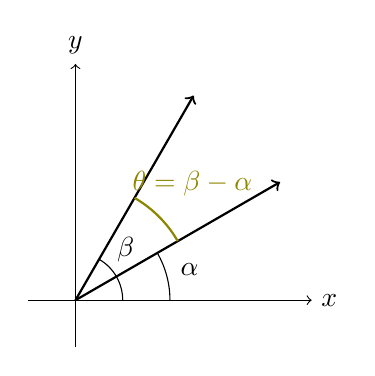
\begin{tikzpicture}[scale=3]
			% Draw axes
			\draw[->] (-0.2, 0) -- (1, 0) node[right] {$x$};
			\draw[->] (0, -0.2) -- (0, 1) node[above] {$y$};

			% Draw angle beta
			\draw[->, thick, black] (0,0) -- (30:1cm);
			\draw[->, thick, black] (0,0) -- (60:1cm);

			% % Mark angles (cosine)
			% Mark arc for be (smaller radius)
			\draw (0.4cm, 0) arc (0:30:0.4cm);  % arc for be (lower)
			\node at (15:0.5cm) {$\alpha$};

			% Mark arc for beta (larger radius)
			\draw (0.2cm, 0) arc (0:60:0.2cm);  % arc for beta
			\node at (45:0.3cm) {$\beta$};

			% Mark arc for theta (same radius as beta)
			\draw[thick, olive] (30:0.5cm) arc (30:60:0.5cm);  % arc for theta from be to beta
			\node[olive] at (45:0.7cm) {$\theta = \beta - \alpha $};

		\end{tikzpicture}
		\caption{Visualization of $\cos(\beta - \alpha) = \cos(\theta)$ in the unit circle.}
	\end{figure}

	\noindent\textnormal{For unit vectors, $\cos \theta = v \cdot w$.
		When $v$ and $w$ are not unit vectors, divide by their length to get $u = v/\|v\|$ and $U = u/\|u\|$ and turn them into unit vectors.}
\end{example}


\label{sec:vectors_and_linear_combination_end}

\clearpage

\chapter{Solving Linear Equations $Ax=b$}
\noindent A systematic way to solve the equation $Ax=b$:
\begin{enumerate}
    \item Apply elimination to $Ax=b$
    \item Get upper triangular $U$
    \item Solve $Ux=c$ by back substitution
\end{enumerate}

\section{The number of solutions to $Ax=b$}

\paragraph{1. Exactly one solution} $A$ has independent columns. $A$ has an inverse matrix $A^{-1}$. Example:

\[
    A =
    \begin{bmatrix}
        2 & 3 \\
        4 & 2
    \end{bmatrix},
    \quad
    b =
    \begin{bmatrix}
        5 \\ 6
    \end{bmatrix}
    \quad\Rightarrow\quad
    x =
    \begin{bmatrix}
        1 \\ 1
    \end{bmatrix}
\]

\paragraph{2. No solution} $b$ is not in the column space of $A$. Example:

\[
    A =
    \begin{bmatrix}
        2 & 3 \\
        4 & 6
    \end{bmatrix},
    \quad
    b =
    \begin{bmatrix}
        6 \\ 15
    \end{bmatrix}
    \quad\Rightarrow\quad
    0=3
\]

\paragraph{3. Infinitely many solutions} $A$ has dependent columns. Example:

\[
    A=
    \begin{bmatrix}
        2 & 3 \\
        4 & 6
    \end{bmatrix},
    \quad
    b=
    \begin{bmatrix}
        6 \\ 12
    \end{bmatrix}
    \quad\Rightarrow\quad
    x=
    \begin{bmatrix}
        3\alpha \\ 6-2\alpha
    \end{bmatrix}
    \text{for any number} \; \alpha
\]

\section{Elimination Matrix $E_{ij}$}

We move column by column from left to right. Typically, the first non-zero element in each column is chosen as the pivot (one row below the row of the pivot we just used).
The pivots are used to eliminate the elements below them.
The elimination matrix $E_{ij}$ eliminates the element $a_{ij}$ in the $i$th row and $j$th column.


\begin{examplex}
    \[
        A =
        \begin{bmatrix}
            2 & 3  & 4  \\
            4 & 11 & 14 \\
            2 & 8  & 17
        \end{bmatrix},
        \quad
        b =
        \begin{bmatrix}
            19 \\ 55 \\ 50
        \end{bmatrix}
    \]

    \paragraph{Step 1}
    The first pivot is $a_{11} = 2$. Eliminate the elements below it. \\
    \vspace{0.4cm}
    Eliminate $a_{21}$ \qquad
    $
        E_{21} =
        \begin{bmatrix}
            1  & 0 & 0 \\
            -2 & 1 & 0 \\
            0  & 0 & 1
        \end{bmatrix}
        \quad
        E_{21}A =
        \begin{bmatrix}
            2 & 3 & 4  \\
            0 & 5 & 6  \\
            2 & 8 & 17
        \end{bmatrix}
        \quad
        E_{21}b =
        \begin{bmatrix}
            19 \\ 17 \\ 50
        \end{bmatrix}
    $

    \vspace{0.4cm}
    Eliminate $a_{31}$ \qquad
    $
        E_{31} =
        \begin{bmatrix}
            1  & 0 & 0 \\
            0  & 1 & 0 \\
            -1 & 0 & 1
        \end{bmatrix}
        \quad
        E_{31}E_{21}A =
        \begin{bmatrix}
            2 & 3 & 4  \\
            0 & 5 & 6  \\
            0 & 5 & 13
        \end{bmatrix}
        \quad
        E_{31}E_{21}b =
        \begin{bmatrix}
            19 \\ 17 \\ 31
        \end{bmatrix}
    $

    \paragraph{Step 2}
    The second pivot is $a_{22} = 5$. Eliminate the elements below it. \\

    \vspace{0.4cm}
    Eliminate $a_{32}$ \qquad
    $
        E_{32} =
        \begin{bmatrix}
            1 & 0  & 0 \\
            0 & 1  & 0 \\
            0 & -1 & 1
        \end{bmatrix}
        \quad
        E_{32}E_{31}E_{21}A =
        \begin{bmatrix}
            2 & 3 & 4 \\
            0 & 5 & 6 \\
            0 & 0 & 7
        \end{bmatrix}
        \quad
        E_{32}E_{31}E_{21}b =
        \begin{bmatrix}
            19 \\ 17 \\ 7
        \end{bmatrix}
    $

    \paragraph{Step 3}
    Solve $Ux=c$ by back substitution. \\

    \vspace{0.4cm}
    Now we have $U = \begin{bmatrix}
            2 & 3 & 4 \\
            0 & 5 & 6 \\
            0 & 0 & 7
        \end{bmatrix}$
    and $c = \begin{bmatrix}
            19 \\ 17 \\ 7
        \end{bmatrix}$. We can go from the bottom up to solve for $x$.
\end{examplex}

\begin{mdframed}
    \textbf{An easy way to come up with elimination matrix} \\

    \noindent To go from $A =
        \begin{bmatrix}
            2 & 3 & 4  \\
            0 & 5 & 6  \\
            2 & 8 & 17
        \end{bmatrix}$ to $B =
        \begin{bmatrix}
            2 & 3 & 4  \\
            0 & 5 & 6  \\
            0 & 5 & 13
        \end{bmatrix}$, we need to come up with $E_{31}$: \\

    \baselineskip=1.5\baselineskip
    \noindent \textbf{1. For the first row in $E_{31}$:} \\
    $A_{row_{1}}$ is $\begin{bmatrix}
            2 & 3 & 4
        \end{bmatrix}$, $B_{row{1}}$ is $\begin{bmatrix}
            2 & 3 & 4
        \end{bmatrix}$. We take $1 \times A_{row_{1}}$, $0 \times A_{row_{2}}$, and $0 \times A_{row_{3}}$. So the first row of $E_{31}$ is $\begin{bmatrix}
            1 & 0 & 0
        \end{bmatrix}$. \\
    \noindent \textbf{2. For the second row in $E_{31}$:} \\
    $A_{row_{2}}$ is $\begin{bmatrix}
            0 & 5 & 6
        \end{bmatrix}$, $B_{row{2}}$ is $\begin{bmatrix}
            0 & 5 & 6
        \end{bmatrix}$. We take $0 \times A_{row_{1}}$, $1 \times A_{row_{2}}$, and $0 \times A_{row_{3}}$. So the second row of $E_{31}$ is $\begin{bmatrix}
            0 & 1 & 0
        \end{bmatrix}$. \\
    \noindent \textbf{3. For the third row in $E_{31}$:} \\
    $A_{row_{3}}$ is $\begin{bmatrix}
            2 & 8 & 17
        \end{bmatrix}$, $B_{row{3}}$ is $\begin{bmatrix}
            0 & 5 & 13
        \end{bmatrix}$. We take $-1 \times A_{row_{1}}$, $0 \times A_{row_{2}}$, and $1 \times A_{row_{3}}$. So the third row of $E_{31}$ is $\begin{bmatrix}
            -1 & 0 & 1
        \end{bmatrix}$. \\
    \noindent \textbf{4. Put it togeter:}
    \[
        E_{31} =
        \begin{bmatrix}
            1  & 0 & 0 \\
            0  & 1 & 0 \\
            -1 & 0 & 1
        \end{bmatrix}
    \]
\end{mdframed}

\section{Permutation Matrix $P$}


\end{document}
